\section{模型建立}    
    \subsection{问题一}
        附件1中所给的数据有部分异常,为了能够继续后续的分析,我们有必要对
        数据进行处理。我们具体使用到的模型是$3\sigma$模型
        模型介绍:数据需要服从正态分布。在$3\sigma$原则下,异常值如
        超过$3$倍标准差,那么可以将其视为异常值。正负$3\sigma$的概率是$99.7\%$
        ,那么距离平均值$3\sigma$之外的值出现的概率为
        $P(|x-u| 3\sigma) = 0.003$,
        属于极个别的小概率事件。如果数据不服从正态分布,也可以用远离平均
        值的多少倍标准差来描述。概率分布如下表
        \begin{table}[H]
            \centering
            \begin{tabular}{|c|c|}
                \hline
                数值分布&在数据中的占比\\
                \hline
                $(\mu-\sigma,\mu+\sigma)$&$0.6827$\\
                \hline
                $(\mu-2\sigma,\mu+2\sigma)$&$0.9545$\\
                \hline
                $(\mu-3\sigma,\mu+3\sigma)$&$0.9973$\\
                \hline
            \end{tabular}
            \caption{常用的$\sigma$分布表}
        \end{table}
        我们可以检测这一段时间的统计数据,假如符合正态分布,计算
        均值$M$与标准差$\sigma$。如果后来的统计值$C$不在这个范围$3\sigma$
        范围内,就可以认为这个值是异常值。
        根据模型的思路,我们首先计算出平均值与标准差,遍历每个管道的各种数据,
        得到计算均值$M$与标准差$\sigma$
        如果管道温度$\mathbb{C}$超过异常值,即满足
        \begin{equation}
            \begin{aligned}
                \mathbb{C} > 3\sigma + M \\
                \mathbb{C} < 3\sigma + M  \\
            \end{aligned}
        \end{equation}
        则用平均值$M$代替,这样我们得到了所有处理完的数据。
        为了能够细化地概括管道的温度曲线特征,我们可以通过绘制数据图表观察
        综合走势,确定整体印象。
    

        \begin{figure}[H]
            \centering
            \begin{subfigure}{0.32\textwidth}
                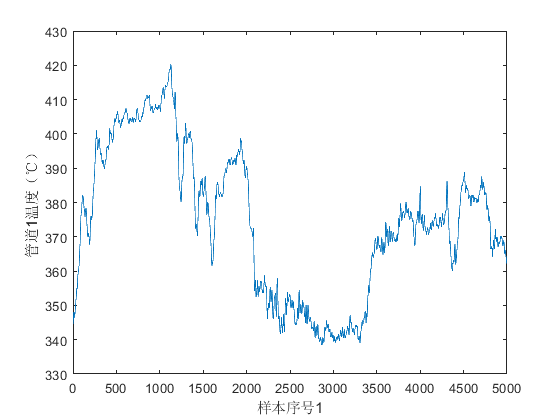
\includegraphics[width=\textwidth]{figures/p1_1.png}
                \label{p1_1}
                \caption{管一}
            \end{subfigure}
            \begin{subfigure}{0.32\textwidth}
                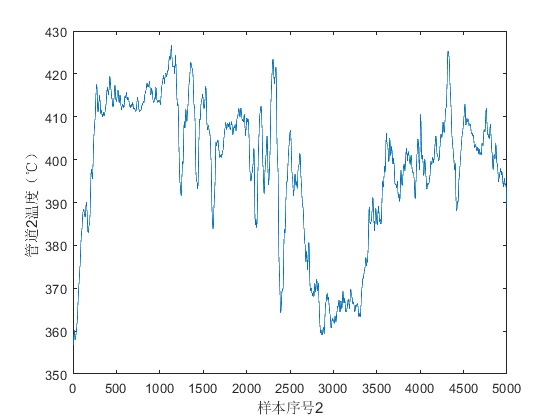
\includegraphics[width=\textwidth]{figures/p1_2.png}
                \label{p1_2}
                \caption{管二}
            \end{subfigure}
            \begin{subfigure}{0.32\textwidth}
                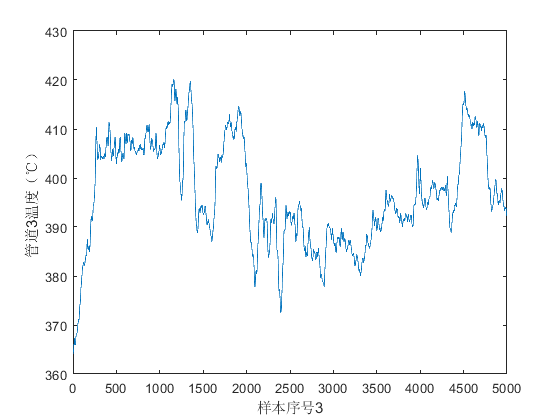
\includegraphics[width=\textwidth]{figures/p1_3.png}
                \label{p1_3}
                \caption{管三}
            \end{subfigure}
            \begin{subfigure}{0.32\textwidth}
                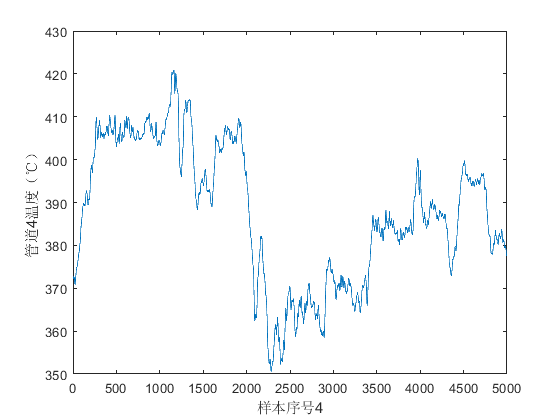
\includegraphics[width=\textwidth]{figures/p1_4.png}
                \label{p1_4}
                \caption{管四}
            \end{subfigure}
            \begin{subfigure}{0.32\textwidth}
                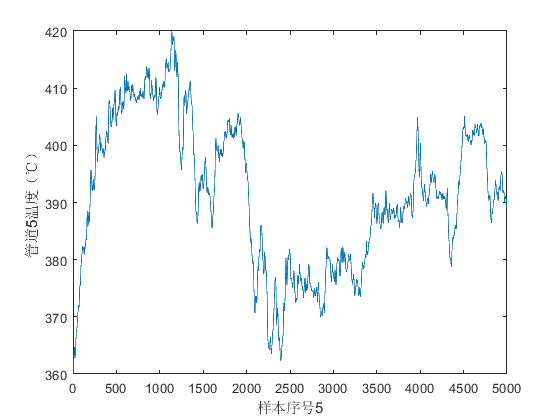
\includegraphics[width=\textwidth]{figures/p1_5.png}
                \label{p1_5}
                \caption{管五}
            \end{subfigure}
            \begin{subfigure}{0.32\textwidth}
                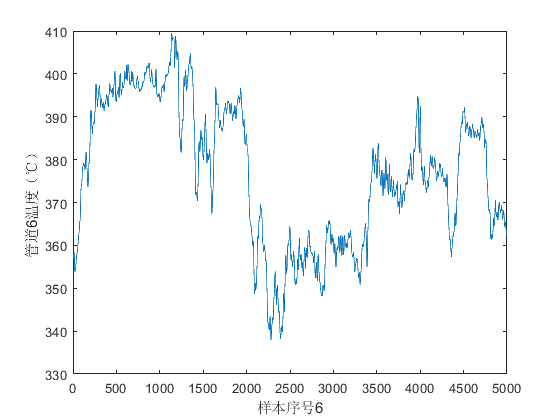
\includegraphics[width=\textwidth]{figures/p1_6.png}
                \label{p1_6}
                \caption{管六}
            \end{subfigure}
        \end{figure}

        \setcounter{figure}{0}%前面的图没有标号,这里置0包括两个图
        \begin{figure}[H]
            \centering
            \setcounter{subfigure}{6}%这里续上之前的6个小图
            \begin{subfigure}{0.40\textwidth}
                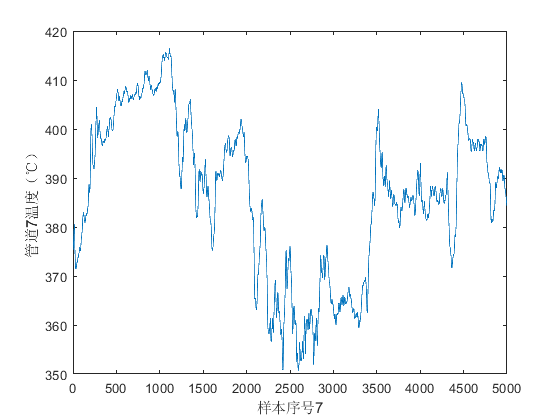
\includegraphics[width=\textwidth]{figures/p1_7.png}
                \label{p1_7}
                \caption{管七}
            \end{subfigure}
            \begin{subfigure}{0.40\textwidth}
                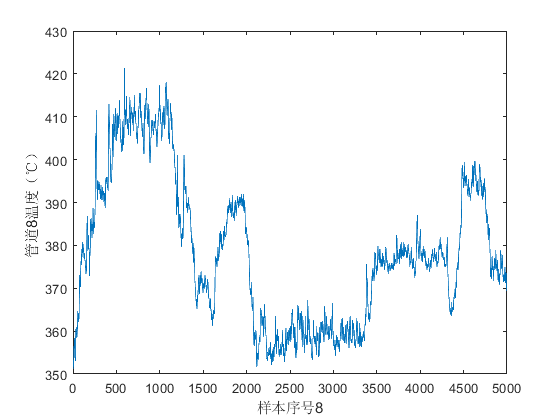
\includegraphics[width=\textwidth]{figures/p1_8.png}
                \label{p1_8}
                \caption{管八}
            \end{subfigure}
            \begin{subfigure}{0.40\textwidth}
                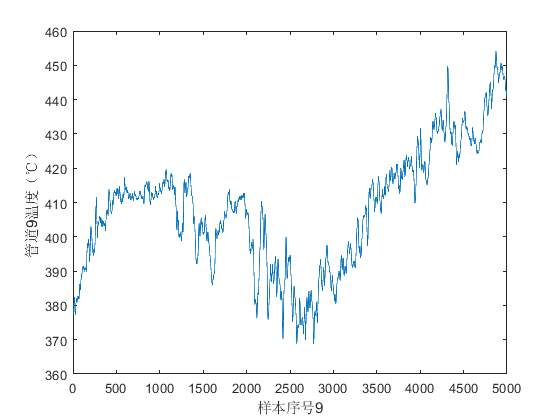
\includegraphics[width=\textwidth]{figures/p1_9.png}
                \label{p1_9}
                \caption{管九}
            \end{subfigure}
            \begin{subfigure}{0.40\textwidth}
                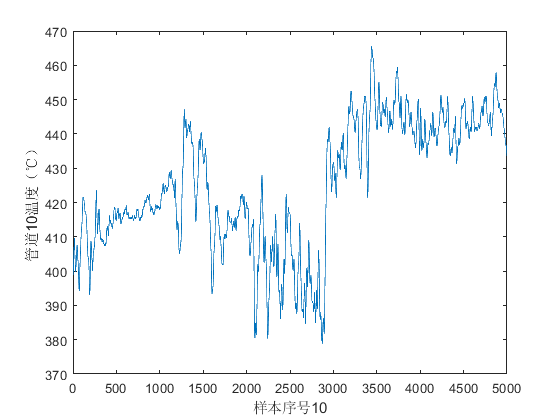
\includegraphics[width=\textwidth]{figures/p1_10.png}
                \label{p1_10}
                \caption{管十}
            \end{subfigure}
            \caption{所有的温度图}
        \end{figure}
        为了能够更清晰地了解温度图像的细节,我们继续计算
        每个管道的平均值$M_i$,标准差$\sigma_i$,方差$\sigma_i^2$,
        最大值$\max_i$和最小值$\min_i$来综合判断。
        \begin{table}[H]
            \centering
            \begin{tabular}{ c|c|c|c|c|c|c|c|c|c|c  }
                \hline
                %\multicolumn{4}{|c|}{Country List} \\                                             
                &管一&管二&管三&管四&管五&管六&管七&管八&管九&管十\\
                \hline
                平均值&374.3&  397.9& 396.7  &387.6 & 391.3 & 376.8  &386.1 & 378.6 & 408.0 & 424.9\\
                标准差&21.4 &  16.8 &  10.6 &  16.3 &  12.9 &  16.6  & 16.0  & 17.2 & 17.7  & 18.6 \\
                方差  &460.0& 283.9 & 113.9  &268.1 & 168.3 & 277.3 & 256.6 & 296.1 & 313.4 & 349.3\\
                最大值&420.2& 426.6 & 420.2 & 420.9 & 419.9 & 409.5 & 416.5 & 421.3 & 454.3 & 465.4\\
                最小值&338.6& 356.8 & 364.2 & 350.6 & 360.00& 338.0& 350.6 & 351.2 & 368.7 & 378.8 \\
                \hline
            \end{tabular}
            \caption{管温度总览}
        \end{table}
        这样问题一的温度趋势变化特点就非常清晰了,以下是我们最后得到的表格:
        \begin{table}[H]
            \centering
            \begin{tabular}{ |p{2.5cm}<{\centering}|p{2.5cm}<{\centering}|p{2.5cm}<{\centering}|p{2.5cm}<{\centering}|p{2.5cm}<{\centering}|  }
                \hline
                %\multicolumn{4}{|c|}{Country List} \\                                             
                $0-1000$&$1000-2000$&$2000-3000$&$3000-4000$&$4000-5000$\\
                \hline
                迅速向上,到达最高点后减缓&
                迅速降温,中途反弹,随后继续降温&
                继续降温直到最低点,缓慢上升一点&
                缓慢上升,中间震荡较多&
                温度趋于平稳,在区间内震荡\\
                \hline
            \end{tabular}
            \caption{趋势表}
        \end{table}


    \subsection{问题二}
        \subsubsection{$TOPSIS$优劣解距离法模型}
        目前对指标的优劣性评价方法有很多,如模糊综合评价法、层次分析法、模糊综
        合评价等,这些方法各具特色。而$TOPSIS$法能够降低主观因素的干扰,应用灵
        活且计算简便,将其应用于管道的温度曲线平稳性评估,能够得到较客观和准确的结果。
        我们首先提取出$n×m$的$n$个对象,$m$个评价指标的原始矩阵
        ,再将该矩阵进行正向化处理,得到正向化矩阵$A$。
        \begin{equation}
            A=\begin{pmatrix}
                a_{11} & a_{12} & \cdots& a_{1m}\\
                a_{21} & a_{22} & \cdots& a_{2m}\\
                \vdots & \vdots & \ddots& \vdots\\
                a_{n1} & a_{n2} & \cdots& a_{nm}\\
                \end{pmatrix}
        \end{equation}
        再对矩阵$A$进行标准化处理以消除量纲得到矩阵$B$,其中
        \begin{equation}
            b_{ij}=\frac{a_{ij}}{\sqrt{\sum_{n = 1}^{\infty} a_{ij}  }}
        \end{equation}
        我们分别定义最大值$B_+$和最小值$B_-$
        \begin{equation}
            \begin{aligned}
                B^+ = (B_1^+, B_2^+,\cdots, B_n^+)=&(\max \{b_{11},b_{21},\cdots,b_{n1}\},\\
                &max\{b_{12},b_{22},\cdots,b_{n2}\},\cdots,max\{b_{1m},b_{2m},\cdots,b_{nm}\})      
            \end{aligned}
        \end{equation}
        \begin{equation}
            \begin{aligned}
                B^- = (B_1^-, B_2^-,\cdots, B_n^-)=&(\min \{b_{11},b_{21},\cdots,b_{n1}\},\\
                &min\{b_{12},b_{22},\cdots,b_{n2}\},\cdots,min\{b_{1m},b_{2m},\cdots,b_{nm}\})
            \end{aligned}
        \end{equation}
        于是,我们分别计算出第i个评价对象与最大、最小值的距离$D_i^+$,$D_i^-$,
        \begin{equation}
            D_i^+ = \sqrt{\sum_{j=1}^{m} (B_j^+ - b_{ij})^2}
        \end{equation}
        \begin{equation}
            D_i^- = \sqrt{\sum_{j=1}^{m} (B_j^- - b_{ij})^2}
        \end{equation}
        据此,我们可以得到第$i(i=1,2,…,n)$个评价对象的得分$W_i$
        \begin{equation}
            W_i = \frac{D_i^-}{D_i^+ - D_i^-}
        \end{equation}
        最后我们将得分$W_i$归一化即可得到归一化后的得分$\tilde{W_i}$
        \begin{equation}
            \tilde{W_i} = \frac{W_i}{\sum_{i=1}^{n} W_i}
        \end{equation}
        根据归一化后得分的高低,我们可以对水冷壁管道温度数据曲线评估
        并排序,确定其中的最优工作曲线和最劣工作曲线。

        \subsubsection{模型展开}
            我们组确定各个管道的温度数据作为曲线平稳度评价指标所对应
            的数据,并应用$TOPSIS$模型对数据进行处理。
            根据$TOPSIS$模型中的公式,我们可以得到对
            10个管道温度曲线平稳度的综合得分。
        \subsubsection{模型解决}
            根据模型。我们建立评价函数。令445为最大值,如果超过最大值,则降低评价分数
            这里我们就直接将温度设定成1000,这样会极大地降低其对应的评价分数。\par
            首先对矩阵原数据矩阵$A$进行标准化,得到新的矩阵$B$。
            \begin{equation}
                A=\begin{pmatrix}
                    0& 579.80\\
                    176.14&	573.40\\
                    346.13&	579.80\\
                    191.97&	579.10\\
                    291.70&	580.10\\
                    182.69&	590.50\\
                    203.44&	583.50\\
                    163.94&	578.70\\
                    146.63&	0\\
                    110.69&	0\\
                \end{pmatrix}
                B=\begin{pmatrix}
                    0	  &  0.3530\\
                    0.2757&	0.3491\\
                    0.5417&	0.3530\\
                    0.3004&	0.3526\\
                    0.4565&	0.3532\\
                    0.2859&	0.3595\\
                    0.3184& 0.3553\\
                    0.2566&	0.3523\\
                    0.2295&	0\\
                    0.1732&	0\\
                \end{pmatrix}
            \end{equation}
            由上图可知,管道的温度曲线平稳度得分如下表
            \begin{table}[H]
                \begin{tabular}{|c|c|c|c|c|c|c|c|c|c|}
                    \hline
                    管一&管二&管三&管四&管五&管六&管七&管八&管九&管十\\
                    \hline
                    0.0652 &0.1035 &0.1638 &0.1087&0.1441
                    &0.1062&0.1127&0.1000&0.0538&0.0416\\
                    \hline
                \end{tabular}
                \caption{管道平稳度得分}
            \end{table}
            由此,我们可以知道管三的平稳度得分最高,为0.1638分。
            而最差的是管10,只有0.0416分。结合图表也可以发现,
            管10的温度曲线震动幅度最大,而且有相当长的一段时间是
            位于445度以上。
    \subsection{问题三}
        \subsubsection{模型建立}
        对附件2的153个回归自变量$X_1,X_2,\cdots,X_{153}$,分别同因变量
        $Y$建立一元回归模型
        \begin{equation}
            Y = \beta_0 + \beta_iX_i + \epsilon, i = 1,2,\cdots, 153
        \end{equation}
        计算变量$X_i$,相应的回归系数的F检验统计量的值,
        记为$F_1^{(1)},\cdots,F_p^{(1)}$,取其中的最大值$F_{i_1}^{(1)}$,即
        对给定的显著性水平$\alpha$,记相应的临界值为$F^(1)$,
        $F_{i_1}^{(1)} \geqslant F^{(1)}$,则将$X_{i_1}$引入回归模型,记
        $I_1$为选入变量指标集合。\par
        步骤2:建立因变量$Y$与自变量子集$\{X_{i_1},X_1\},\cdots,
        \{X_{i_1},X_{i_1-1}\},\{X_{i_1},X_{i_1+1}\},\cdots,$
        $\{X_{i_1},X_{153}\}$
         的二元回归模型(即此回归模型的回归元为二元的),共有152个。计算变量的回
        归系数$F$检验的统计量值,记为$F_k^{(2)}(k\notin I_1)$,
        选其中最大者,记为 $F_{i_2}^{(2)}$
        ,对应自变量脚标记为$i_2$,即
        \begin{equation}
            F_{i_2}^{(2)} = \max \{F_1^{(2)},\cdots,F_{152}^{(2)},F_{153}^{(2)} \}
        \end{equation}
        对给定的显著性水平 ,记相应的临界值为$F^{(2)}$ ,$F_{i_2}^{(2)} \geqslant F^{(2)}$ 
        则变量$X_{i_2}$引入回归模型。否则,终止变量引入过程\par
        步骤3:考虑因变量对变量子集  $\{X_{i_1},X_{i_2},X_K\}$的回归重复步骤2。
        依此方法重复进行,每次从未引入回归模型的自变量中选
        取一个,直到经检验没有变量引入为止。\par
        在进行完逐步回归模型之后,我们分别对各个管道得到了影响度较大的变量。
        随后,我们对剩下的变量分别进行线性回归分析,得到了较好的拟合度。
        \subsubsection{问题解决}
            使用附件二中的152个变量,通过$matlab$的$stepwisefit()$
            函数进行逐步回归分析,
            每个管道都得到了相关的变量。变量的因子分布如图分布:
            \begin{figure}[H]
                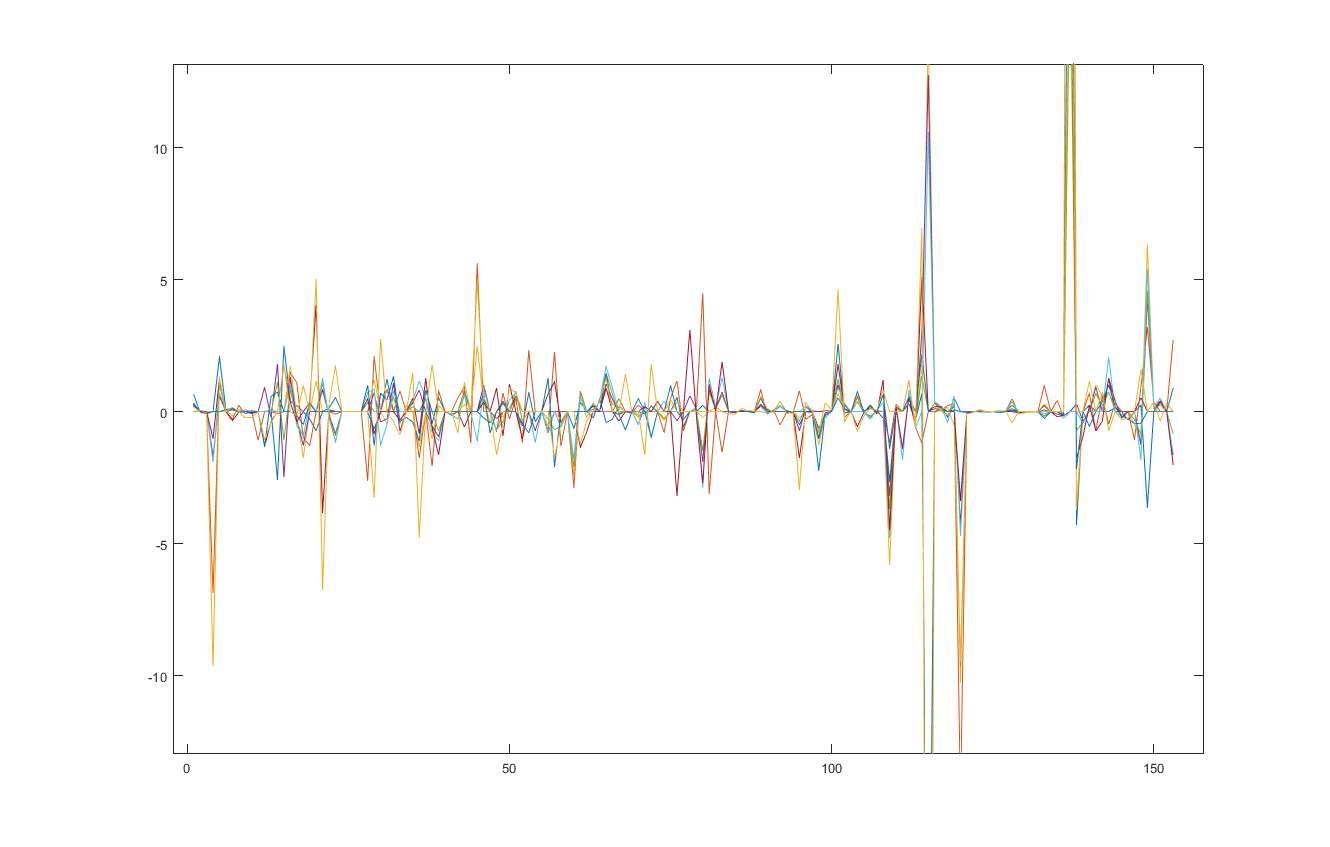
\includegraphics{变量因子分布.bmp}
                \caption{变量因子权重分布图}
            \end{figure}
            \begin{table}[H]
                \centering
                \begin{tabular}{|c|c|c|c|c|c|c|c|c|c|c|}
                    \hline
                    管道名&管一&管二&管三&管四&管五&管六&管七&管八&管九&管十\\
                    \hline
                    变量数&78&91&85&91&91&93&90&72&90&90\\
                    \hline
                \end{tabular}
                \caption{逐步回归所保留的变量}
            \end{table}
            由于每个管道的变量因子数过多,我们为了后续更好的分析,需要舍弃部分
            权重较小的变量。所以我们选取前10个权重最大的变
            量作为之后线性回归的参量。\par
            剩下选取的十个管道对应的变量如表所示
            \begin{table}[H]
                \centering
                \begin{tabular}{|c|c|c|c|c|c|c|c|c|c|c|}
                    \hline
                    管道名&管一&管二&管三&管四&管五&管六&管七&管八&管九&管十\\
                    \hline
                    位置1&78&91&85&91&91&93&90&72&90&90\\
                    \hline
                    位置2&78&91&85&91&91&93&90&72&90&90\\
                    \hline
                    位置3&78&91&85&91&91&93&90&72&90&90\\
                    \hline
                    位置4&78&91&85&91&91&93&90&72&90&90\\
                    \hline
                    位置5&78&91&85&91&91&93&90&72&90&90\\
                    \hline
                    位置6&78&91&85&91&91&93&90&72&90&90\\
                    \hline
                    位置7&78&91&85&91&91&93&90&72&90&90\\
                    \hline
                    位置8&78&91&85&91&91&93&90&72&90&90\\
                    \hline
                    位置9&78&91&85&91&91&93&90&72&90&90\\
                    \hline
                    位置10&78&91&85&91&91&93&90&72&90&90\\
                    \hline
                \end{tabular}
                \caption{十个管道分别对应的十个变量位置}
            \end{table}
            随后,通过$matlab$自带的$regress()$函数,
            对指定的变量分别进行线性回归分析,得到了各个拟合度:
            \begin{table}[H]
                \centering
                \begin{tabular}{|c|c|c|c|c|c|c|c|c|c|c|}
                    \hline
                    管道名&管一&管二&管三&管四&管五&管六&管七&管八&管九&管十\\
                    \hline
                    拟合度&0.9545&0.9742&0.9718&0.9746&0.9783&0.9825&0.9609&0.9474&0.9545&0.9911\\
                    \hline
                \end{tabular}
                \caption{拟合度表格}
            \end{table}
            可以发现我们所选取的变量进行线性回归后,拟合度均在$95\%$以上
            效果非常好
    \subsection{问题四}
        第四题分析超温现象的原因。我们在第三题中已经找到了十个权重较大的变量,
        这些变量很有可能是导致第十个超温变化的原因。
        观察图片可以发现
        \begin{figure}[H]
            \centering
            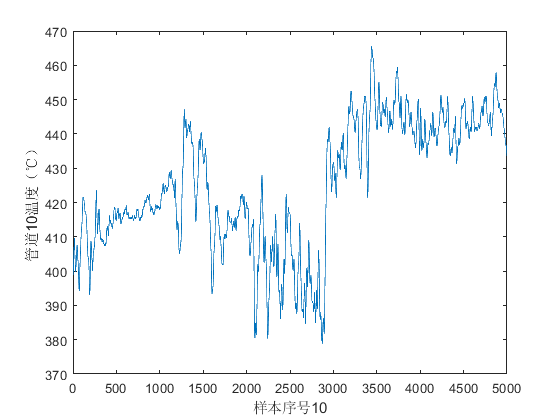
\includegraphics[width=0.8\textwidth]{figures/p1_10.png}
            \caption{管十的温度曲线图}
        \end{figure}
        其中管道的温度在1800-2400时间段是位于一个较低的区间,整体来说比较稳定,
        因此其变量都有一个统一的特征。而3147之后的温度则位于一个统一较高的区间,
        总体来说也比较稳定,因此变量也应该拥有一个相同的特征。
        我们先确定分界点为$S=3147$,位于分界点$S$之前的变量特征为$S_{low}$,
        位于分界点$S$之前的变量特征为$S_{high}$。每10组温度数据分为一组,计算
        其变量特征的平均值$S_{low_i}$与$S_{high_i}$。令两个变量特征的
        平均值为
        \begin{equation}
            \Delta X_i = |S_{low_i} - S_{high_i}|
        \end{equation}
        总共计算20次,经过了$20\times 10 \times 2 = 400$组数据,
        具有较好的统计价值。我们汇总所有的$\Delta X_i$值,
        如图(\ref{delta_x_distribution})
        \begin{table}
            \centering
            \begin{tabular}{|c|c|c|c|c|c|c|c|c|c|c|}
                \hline
                管道名&管一&管二&管三&管四&管五&管六&管七&管八&管九&管十\\
                \hline
                拟合度&0.9545&0.9742&0.9718&0.9746&0.9783&0.9825&0.9609&0.9474&0.9545&0.9911\\
                \hline
            \end{tabular}
            \caption{$\Delta X_i$分布图}
            \label{delta_x_distribution}
        \end{table}
        随后,统计各变量的分布图,如图(\ref{4_variable_frequency})
        \begin{figure}

            \label{4_variable_frequency}
            \caption{变量出现频率柱状图}
        \end{figure}

    \subsection{问题五}
        问题五的分析。。。。    